\documentclass{article}

\usepackage[utf8]{inputenc}
\usepackage{graphicx}
\usepackage[german]{babel}
%\usepackage{algorithm}
%\usepackage{algorithmic}
\usepackage{cite}

\setlength{\parindent}{0pt}

\title{Proteinsequenz-Vergleich mit KSEARCH und SANS}
\author{Meike Bruns, Florian Markowsky, Michael Spohn}

\begin{document}

\maketitle
\thispagestyle{empty}
\begin{abstract}
\end{abstract}
\newpage

\tableofcontents
\thispagestyle{empty}
\newpage

\section{Einleitung: Sequenzvergleiche}

Eine bei der Sequenzanalyse am häufigsten anfallenden Aufgaben ist der Vergleich von Sequenzen. Sowohl bei DNA als auch bei Proteinsequenzen können
durch Sequenzvergleich gefundene, ähnliche Sequenzen oder Sequenzfamilien Aufschluss über Verwandschaftsbeziehungen, konservierte Regionen und zahlreiche
andere Eigenschaften einer betrachteten Sequenz geben. Da der exakte Sequenzvergleich, beispielsweise durch die Suche von Alignments per Smith-Waterman
Algorithmus (\cite{Water}), sehr zeitaufwändig ist, bedient man sich meist schnellerer, nicht-axakter Methoden. Hier ist besonders der BLAST-Algorithmus (\cite{BLAST})
zu erwähnen, der sich als de-facto Standart etabliert hat.
%TODO mehr blalba?

Im folgenden werden wir zwei Familien von Sequenzvergleich-Algorithmen und ihre wichtigsten Vertreter kurz vorstellen.
\begin{itemize}
  \item Aligmentbasierte Methoden
    \begin{itemize}
      \item SSEARCH: Der SSearch-ALgorithmus führ ein Alignment der Query- und der Datenbanksequenzen durch. %TODO Algorithmen kurz erklären
      \item FASTA
      \item BLAST
    \end{itemize}
  \item Ranking mittels Feature-Vektoren
    \begin{itemize}
      \item USearch
      \item KSearch
      \item SANS
    \end{itemize}
\end{itemize}

\section{Algorithmen \& Implementierung}

\subsection{Datenstrukturen}

\subsubsection{Hashes}%TODO erklären wir das? rot-schwarz bäume auch?

\subsubsection{Suffix-Arrays}

Ein Suffix-Array ist eine Indexdatenstruktur, die die Indices der lexikographisch geordneten Suffixe eines Strings speichert. %TODO erklären, Quelle: GI-Skript?

\subsection{KSEARCH}
\label{ksearch}

Der in \cite{Holm} vorgestellte KSearch-Algorithmus nutzt als Ähnlichkeitsmaß zweier Sequenzen die Übereinstimmung ihrer kmer-Profile.%TODO KSearch beschreiben

%\begin{algorithm}
%  \caption{Pseudocode unserer KSearch-Implementierung}
%\begin{algorithmic}
%  \Function{KSEARCH}{query-proteins $Q$, database-proteins $D$}
%    \For{each query-protein $q$}  
%      \State calculate kmer-profile \Comment $O(|q|)$
%      \State store kmer-profile in hashtable
%    \EndFor \Comment $\boldsymbol{O(|q_0..q_n|)}$
%    \For{each database-protein $d$} 
%      \State calculate kmer-profile \Comment $O(|d|)$
%      \For{i in $Q$}
%        \State calculate $KSEARCH(d,q_{i})$ \Comment $O(kVariety(d))$   
%        \State output $KSEARCH(d,q)$
%      \EndFor \Comment $\boldsymbol{ O(|Q| \cdot kVariety(d))}$
%    \EndFor   \Comment $\boldsymbol{O(|d_0..d_n|+|D| \cdot |Q| \cdot kVariety(d))}$  
%  \EndFunction \Comment overall time complexity: $\boldsymbol{O(|q_0..q_n|+|d_0..d_n|+|D| \cdot |Q| \cdot kVariety(d))}$
%\end{algorithmic}
%\end{algorithm}

\subsection{SANS}
\label{sans}

%TODO Sans beschreiben

\subsection{Software Architektur}

\subsubsection{Genometools}

Wir implementieren unsere Algorithmen als Teil der Genometools, einer Sammlung von Werkzeugen und Klassen zur Genomanalyse (\cite{gtools}).
Im folgenden gehen wir auf die Teile der genometools ein, die wir für unsere Implementierung genutzt haben.
\begin{itemize}
  \item encseq: Ein Tool zur Repräsentation von Biosequenzen.
  \item suffixerator: Ein Tool zur Berechnung von Suffixbäumen aus sequenzdateien oder encseqs.
\end{itemize}

\subsubsection{Struktur}

Da wir zwei verschiedene Algorithmen implementieren, ist eine logische Trennung wichtig. Da beide jedoch eine ähnliche Funktionalität erfüllen und
zumindest teilweise gleiche Strukturen beinhalten, würde eine komplette Trennung auf Code-Redundanzen hinauslaufen. Um dieses Dilemma zu lösen, haben wir
die \emph{Seqscore} Toolbox geschaffen, die die beiden Unter-Tools \emph{KSEARCH} und \emph{SANS} enthält. Diese greifen auf die selbe Codebasis zu, 
\emph{bla\_seqscore.c}. Dabei ruft jedes Tool abhängig von den ihm übergebenen Ausgabeparametern einen Konstruktor in \emph{bla\_seqscore.c} auf. Es gibt also
sechs Konstruktoren, eine je Algorithmus und je gewählter Ausgabe. Siehe dazu Abbildung \ref{seqsc}. Auf diese Weise ist sichergestellt, das die 
Ergebnisstrukturen betreffender Code von beiden Algorithmen genutzt werden kann.

\begin{center}
  \begin{figure}
    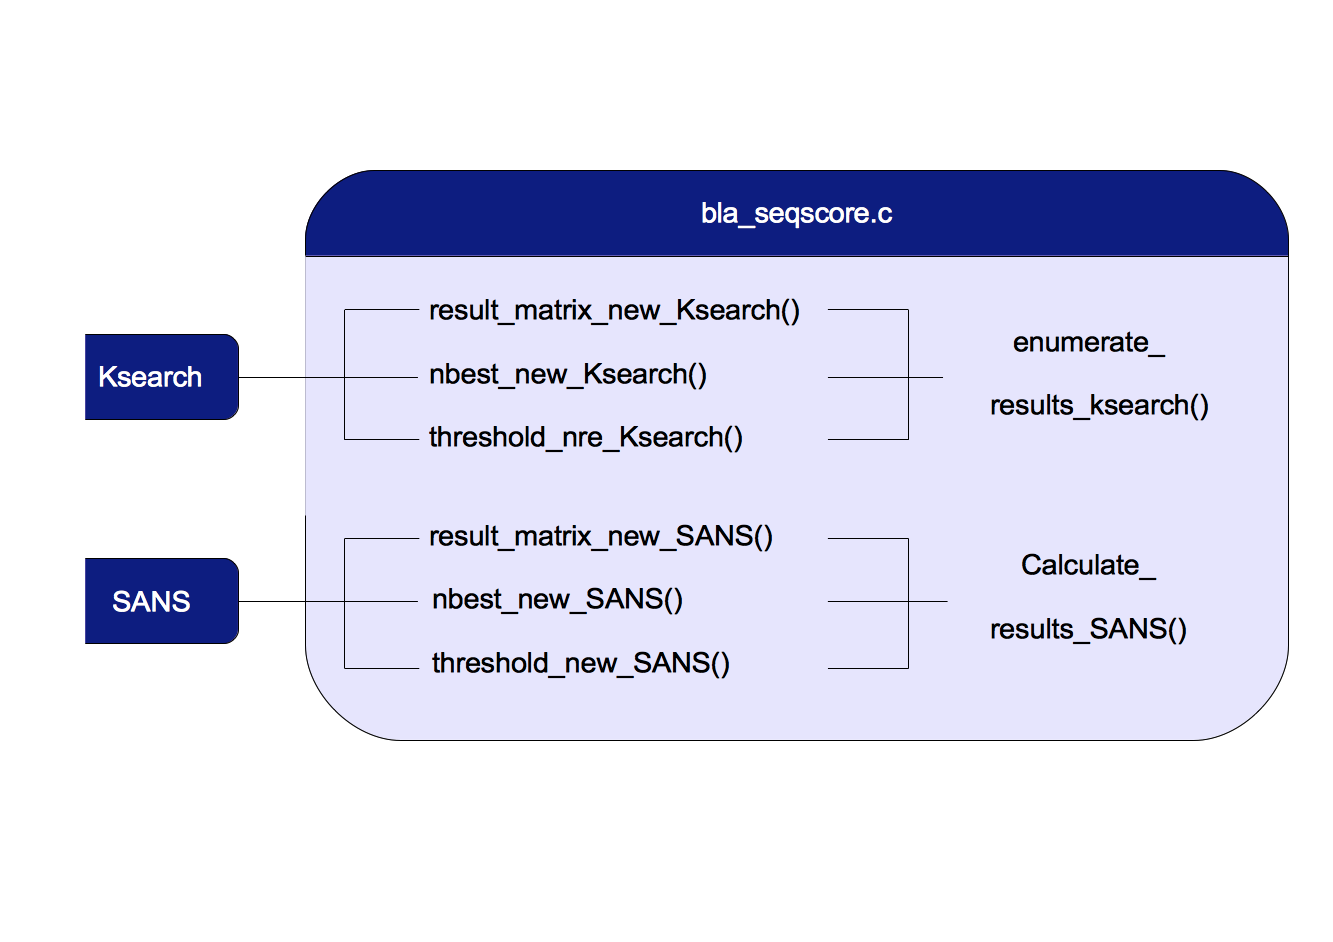
\includegraphics[width = \linewidth]{img/dia2}
    \caption{Struktur der \emph{bla\_seqscore.c}. Pro von Außen aufrufendem Tool sind drei Konstruktoren vorhanden, die jedoch jeweils wieder die
    selbe Berechnungsfunktion ausführen.}
    \label{seqsc}
  \end{figure}
\end{center}

Pro Algorithmus wurde eine tatsächliche Berechnungsfunktion implementiert. Auf diese wird aus den drei Ergebnisstruktur abhängigen Konstruktoren des jeweiligen
Algorithmus zugegriffen. Wir gehen zunächst auf den \emph{SANS} Algorithmus ein.

Da durch die unter Abschnitt \ref{sans} vorgestellte Berechnungsvorschrift der Score für ein Sequenzpaar erst bei der Terminierung des ALgorithmus
fest steht, muss für jeden \emph{SANS} Lauf die gesamte Ergebnismatrix der Dimension $|Q|\cdot|D|$ mitgeführt werden. Die Konstruktoren 
\emph{result\_matrix\_new\_sans()}, \emph{nbest\_new\_sans()} und  \emph{threshold\_new\_sans()} definieren also jeweils die Ergebnismatrix und allokieren
den entsprechenden Speicher und rufen dann die \emph{calculate\_results\_sans()} Funktion auf, die die Matrix füllt. Anschließend werden die Daten 
wiederum Konstruktorspezifisch aufbereitet. Der \emph{matrix}-Konstruktor wird also die gesamte Matrix, der \emph{nbest}-Konstruktor eine
Liste der $n$ besten Scores und der dazugehörigen Sequenzen und der \emph{treshold}-Konstruktor alle Sequenzpaare, deren Score über dem gegebenen
Schwellwert liegt, zurückgeben.

Wie in Abschnitt \ref{ksearch} ersichtlich, kann beim \emph{KSEARCH}-Algorithmus Speicherplatz gespart werden, da die Scores der Sequenzpaare
nacheinander ausgerechnet werden. Es muss also nur wenn der Benutzer die \emph{matrix}-Rückgabe gewünscht hat tatsächlich der Speicher für die
ganze Ergebnismatrix allokiert werden. Dies nutzen wir aus, indem die Konstruktoren \emph{result\_matrix\_new\_ksearch()}, \emph{nbest\_new\_ksearch()} 
und  \emph{threshold\_new\_ksearch()} eine ausgabespezifische Ergebnisstruktur erstellen und neben dieser Struktur auch eine Callback-Funktion an 
die \emph{enumerate\_results\_ksearch()} Funktion übergeben. Wie der Name der Funktion bereits anzeigt, berechnet die Funktion due \emph{KSEARCH}-Scores
sequenziell und ruft für jeden berechneten Score die übergebene Callback Funktion auf. Dieser wird auch die Ergebnisstruktur übergeben, so dass diese
der gewünschten Ausgabe entsprechend gefüllt werden kann. Abbildung \ref{kscallback} zeigt die Aufruf-Reihenfolge und die übergebenen Datenstrukturen am
Beispiel des \emph{result\_matrix\_new\_ksearch} Konstruktors.

\begin{center}
  \begin{figure}
    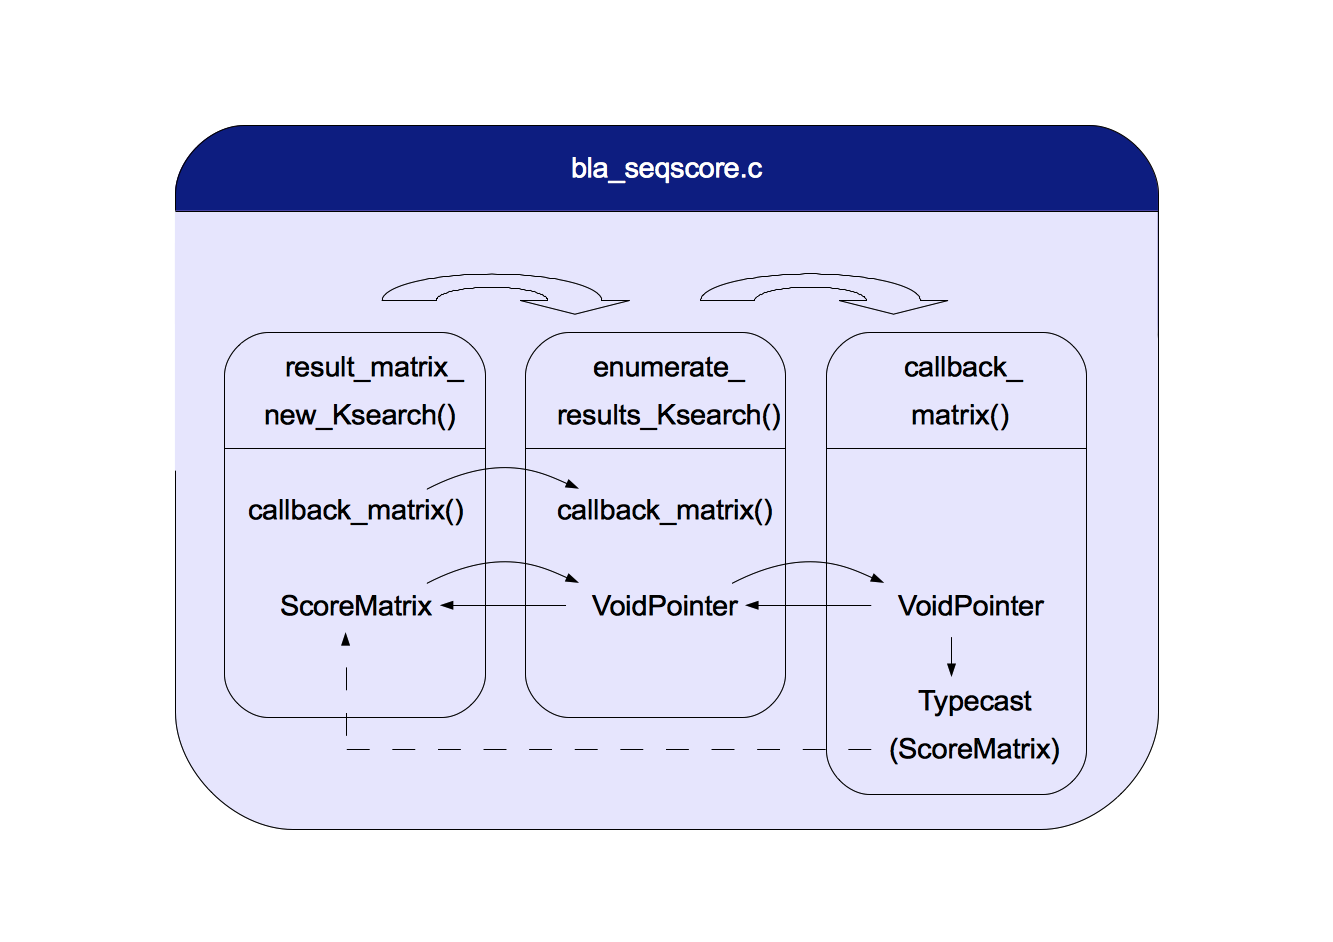
\includegraphics[width = \linewidth]{img/dia3}
    \caption{Aufruf-Reiehenfolge bei Aufruf des \emph{result\_matrix\_new\_ksearch} Konstruktor. Der Konstruktor übergibt der Funktion zur Score-Berechnung
      die Callback-Funktion \emph{callback\_matrix()} sowie die \emph{ScoreMatrix} als Ergebnisstruktur. Erst in der Callback-Funktion, die in der 
      Berechnungsfunktion aufgerufen wird, wird die Ergebnisstruktur wieder zu einer Matrix gecastet und befüllt.}
    \label{kscallback}
  \end{figure}
\end{center}

Für die \emph{matrix}-Option ist diese Rückgabestruktur ein einfaches zweidimensionales Array. Für die \emph{nbest} Option wurde eine in den genometools
bereits vorhandene Implementierung eines Red-Black-Trees als verkettete Liste genutzt. Diese kann schnell prüfen, ob ein neu generierter Score kleiner oder
grüßer als das bisher kleinste Element ist und entsprechend verfahren. Im Falle der \emph{threshold}-Option ist keine Ergebnisstruktur nötig,
da ein berechneter Score, der über dem gegebenen Schwellwert liegt, unmittelbar ausgegeben werden kann.

\section{Auswertung}

Um die erstellten Implementierungen von KSEARCH und SANS zu testen, wurden einerseits Laufzeitvergleiche mit den bereits existierenden Algorithmen aus \cite{Holm}, sowie Trefferquoten-Vergleiche mit bewährten Algorithmen wie SSEARCH und BLAST durchgeführt. Als Query-Datensatz dienten alle 1083 \textit{Rattus rattus}-Proteine aus der NCBI-Datenbank. Als Datenbank wurde die zur Uniprot gehörende Swissprot gewählt, welche ca. 500 000 Proteine enthält.

\subsection{Laufzeiten}

Die, im Vergleich zu SSEARCH und BLAST, sehr guten Laufzeiten aus \cite{Holm} konnten nicht ganz erreicht werden (Tab. 1).\\Für KSEARCH liegt dies mit Sicherheit an der Speicherplatz-effizienteren Implementierung mittels Hashtable (s. Abschnitt ??)...\\Der selbst implementierte SANS-Algorithmus benötigt relativ lange für die Erstellung der Suffix-Arrays, zeigt jedoch, bei zunehmender Fensterbreite \textit h, eine weniger stark ansteigende Laufzeit als der Referenzalgorithmus.\\Mit Ausnahme des selbst implementierten KSEARCH zeigen alle Algorithmen eine signifikante Verbesserung der Laufzeiten um teilweise mehr als 50 \%.
  \begin{table}[h]
    \caption{Laufzeitenvergleich; Holms entspricht den Algorithmen aus \cite{Holm}, MMF kennzeichnet die selbst implementierten Algorithmen; Berechnungen durchgeführt auf: Intel i5, 4*3.4GHz, 32gb RAM, XUbuntu}
    \begin{center}
    \begin{tabular}{lrrr}
    \hline
    Algorithmus & Indexing & Suche & Gesamt\\
    \hline
    BLAST & 0m12s & 27m23s & 27m35s\\
    SSEARCH & - & 60m0s & 60m0s\\
    KSEARCH Holms k6 & 1m29s & 0m14s & 1m43s\\
    KSEARCH MMF k6 & -  & 511m53s & 511m53s\\
    SANS Holms h16 & 1m29s &  0m15s & 1m44s\\
    SANS MMF  h16 & 14m19s & 0m36s & 14m55s\\
    SANS Holms h1000 & 1m29s & 7m7s & 8m36s\\
    SANS MMF  h1000 & 14m19s & 1m56s & 16m15s\\
    \hline
    \end{tabular}
    \end{center}
  \end{table}

\subsection{Scores}

Einerseits wurde hierzu verglichen, wie viele der mit SSEARCH ermittelten Treffer auch mit den jeweiligen Algorithmen wiedergefunden werden konnten; andererseits wurde mittels AUC-Berechnungen die Effizienz der Algorithmen getestet.

\subsubsection{Vergleich mit SSEARCH \& BLAST}

\subsubsection{Area under the curve (AUC)}

Um die Effizienz eines Algorithmus zu ermitteln, wird ein precision-recall-Diagramm erstellt, und daraus die AUC berechnet. Die AUC ist die Fläche unter der Kurve, also das Integral. Das precision-recall-Diagramm erhält man, indem Präzision (precision) $p$ gegen Wiederfindungsrate (recall) $r$ geplottet wird. Um beide Werte zu erhalten, wird als erstes eine Liste \textit l mit einem Referenz-Algorithmus erstellt, und anschließend anhand dieser Liste \textit p und \textit r des zu testenden Algorithmus ermittelt.\\In Liste \textit l wurden alle BLAST-Treffer aus dem Query-Datensatz, welche einen e-Value niedriger als eins aufwiesen, eingetragen. Anschließend wurde mit jedem der ersten 50 Proteine des Query-Datensatzes einzeln eine Suche durchgeführt und die jeweils 50 besten Treffer \textit t ausgegeben. Für diese 50 Treffer wurden dann Präzision (precision) $p = \frac{t_0 ... t_i \in l}{t_0 ... t_i}$ und Wiederfindungsrate (recall) $r = \frac {t_0 ... t_i \in l}{t \in l}$ berechnet und ein precision-recall-Diagramm erstellt. Dabei gibt die Wiederfindungsrate \textit r an, wie viele der richtigen Treffer von \textit t zum Zeitpunkt \textit i bereits gefunden wurden. Die Präzision \textit p gibt die Anzahl der richtigen Treffer, im Verhältnis zu allen zum Zeitpunkt \textit i bereits betrachteten Treffern, an. Da \textit p und \textit r Werte zwischen 0 und 1 annehmen, hat die AUC im besten Fall den Wert 1. Im Allgemeinen nimmt mit zunehmender Wiederfindungsrate die Präzision ab, da bei einem kleinen AUC-Wert viele falsch Positiven Treffer auftreten, bis die maximale Anzahl aller richtig Treffer ermittelt ist. Je kleiner also der Wert für AUC, je ineffizienter ist der Algorithmus.\\Zu beachten ist, dass beim Plotten von \textit p gegen \textit r nur ein Punktdiagramm entsteht. Die darin enthaltenen Punkte können nicht interpoliert werden, wodurch die Kurve für die AUC nur näherungsweise bestimmt werden kann.\\Die Ergebnisse sind in Tab. 2 veranschaulicht.
  \begin{table}[h]
    \begin{center}
    \caption{Werte für die AUC; für die 50 ersten Proteine ; je höher der Wert, je effizienter arbeitet der     Algorithmus}
    \leftskip=-0.5cm
    \begin{tabular}{cccccccc}
      \hline
      \multicolumn{3}{c}{KSEARCH Holmes} & SANS Holmes &\multicolumn{3}{c}{KSEARCH MMF} & SANS MMF\\
      \cline{1-3}\cline{5-7}
      k = 5 & k = 6 & k = 7 & h = 50 & k = 5 & k = 6 & k = 7 & h = 50 \\
      \hline
      0,0000 & 0,0000 & 0,0000 & 0,0000 & 0,9663 & 0,9678 & 0,9677 & 0,9291 \\
      \hline
    \end{tabular}
    \end{center}
  \end{table}

\section{Diskussion}

\addcontentsline{toc}{section}{Literatur}
\bibliography{quellen}{}
\bibliographystyle{unsrt}

\end{document}
